\chapter{Context}
\label{chap:context}

\section{Document Scope}
\label{sec:doc-scope}

This is a summary report covering goals, context, process and process reflections of a Bachelor Thesis project. The project explores different approaches to Optical Character Recognition (OCR) - transcribing images of text into computer readable strings (e.g. \texttt{.png}$\rightarrow$\texttt{.txt}) for North S\'{a}mi, an endangered language in the S\'{a}mi branch of the Uralic family. The motivation is to contribute to the preservation of S\'{a}mi cultural heritage by developing a more lightweight and deployable OCR solution that can be used in resource constrained settings, such as community driven projects, edge deployments and institutions with limited infrastructure.

The thesis work yielded two conference submissions. The full scientific article, titled \textbf{Lightweight OCR in North S\'{a}mi Heritage Digitization for Smart Learning}, in IEEE format, was \emph{accepted} to the International Conference on Information, Intelligence, Systems and Applications (IISA) 2026 (theme: \textit{21st century AI and education}) at the University of the Aegean, Rhodes, Greece. The article addresses the research question \textit{Can a lightweight OCR architecture approach Transformer level accuracy for North S\'{a}mi while enabling practical deployment on modest hardware?}.
An extended abstract of this work, titled \textbf{OCR and Machine Translation Pipeline for Low Resource S\'{a}mi Languages}, was \emph{accepted} to the 15th Scandinavian Conference on Artificial Intelligence (SCAI) 2026 (theme: \textit{AI for Good: Innovation, Ethics, Society}) at the University of Southern Denmark (SDU), Odense, Denmark, and will be presented on June 15th during the poster session.

All the technical details, experiments and scientific claims are covered in the IISA paper. Some sections, such as related work only exist in the scientific article, but some sections are duplicated or expanded on in this report for fuller picture. This report focuses on the \emph{process}: how the project evolved, what was achieved, what was abandoned, and reflections on what worked, what did not, and lessons learned.


\section{S\'{a}mi Languages}

The S\'{a}mi are the indigenous people of the S\'{a}pmi region (Figure~\ref{fig:sapmi-map}), which spans the northern parts of Norway, Sweden, Finland and Russia, with archaeological evidence of habitation in the region for several thousand years~\cite{hansenolsen2014}. From the 17th century onward, Swedish, Danish Norwegian and Russian state expansion brought taxation, Christian missionisation and the suppression of pre-Christian religious practice~\cite{hansenolsen2014,rydving1993}.
In the 19th and 20th centuries this escalated into explicit acts of assimilation: Norwegianization in Norway~\cite{minde2003}, the \textit{nomadskola} system in Sweden~\cite{lantto2010}, boarding schools in Finland~\cite{lehtola2004}, and Soviet collectivisation of the Kola S\'{a}mi~\cite{allemann2013}. After the Alta controversy (1979 to 1981), the protests against the construction of a hydroelectric power plant on the Alta River, more rights were granted to the S\'{a}mi people~\cite{minde2003}. S\'{a}mi parliaments started to operate in all three Nordic countries (Finland's body dates to 1973)~\cite{josefsen2015}, the S\'{a}mi flag was adopted in 1986, and Norway formally apologised for the assimilation policies in 2024~\cite{trcnorway2023,storting2024apology}. However, the legacy of suppression has left the S\'{a}mi languages underrepresented in digital resources, a significant barrier to heritage digitisation and language revitalisation efforts~\cite{enstad2025}.

\begin{figure}[h]
  \centering
  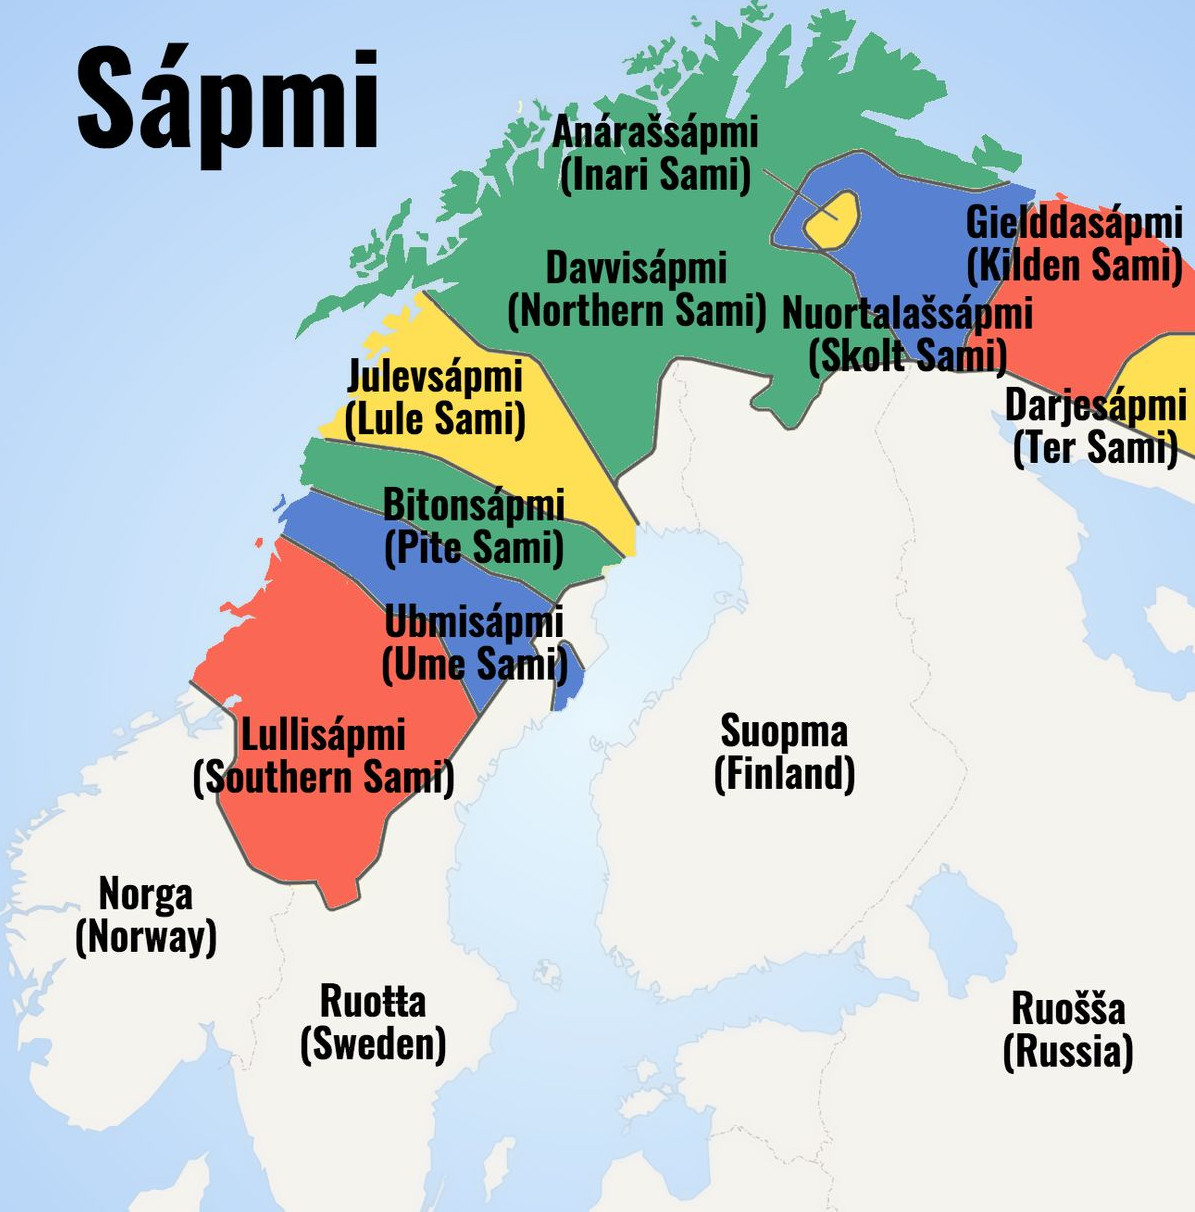
\includegraphics[width=\linewidth]{figures/sapmi1.jpg}
  \caption{The S\'{a}pmi region, spanning the northern parts of Norway, Sweden, Finland and Russia, with the geographic distribution of the nine spoken S\'{a}mi varieties. North S\'{a}mi (\textit{Davvis\'{a}pmi}) covers the largest area. Source: The Decolonial Atlas~\cite{decolonialatlas}, reused under the Decolonial Media License 0.1.}
\label{fig:sapmi-map}
\end{figure}

There are nine mutually unintelligible spoken S\'{a}mi varieties across the S\'{a}pmi region~\cite{sammallahti1998}. The most widely spoken variety, and the focus of this project given the data and tooling available, is North S\'{a}mi (\texttt{ISO 639-3 sme}, \textit{Davvis\'{a}megiella}), with around \smiSpeakers{} speakers, while the most endangered varieties have fewer than 50 speakers, and some are no longer actively spoken~\cite{moseley2010,sammallahti1998}. The S\'{a}mi languages belong to the Uralic family, which also includes Finnish, Estonian and Hungarian~\cite{sammallahti1998}. According to UNESCO's \textit{Atlas of the World's Languages in Danger}~\cite{moseley2010}, North S\'{a}mi is classified as \textit{definitely endangered} (children no longer learn the language as a mother tongue in the home), while the more endangered varieties (Pite, Ter, Ume) are classified as \textit{critically endangered} (the youngest speakers are grandparents and older, who use the language partially and infrequently).

\section{Linguistic Characteristics of North S\'{a}mi}

North S\'{a}mi is an
agglutinative\footnote{
Agglutinative languages build words by stacking distinct morphemes onto a stem, with each suffix typically carrying a single grammatical meaning. For example, North S\'{a}mi \textit{viesuiguin} ``with the houses'' decomposes as \textit{viesu-} (`house') + \textit{-i-} (plural) + \textit{-guin} (`with', the comitative case).}
language with complex morphology and hundreds of inflected\footnote{ Inflection refers to systematic modifications of a word that mark grammatical categories such as case, number, tense, or person. North S\'{a}mi nouns inflect for six cases in singular and plural, while pronouns and verbs additionally distinguish a dual number, yielding many distinct surface forms per stem.}
forms per verb~\cite{valijarvi2013}.
This agglutinative morphology yields large type token ratios even in modest corpora: meaning that the OCR model rarely sees the same exact word twice during training, so it cannot memorise word shapes altogether and is forced to learn the script at the character level. The orthography of North S\'{a}mi further complicates this by including seven special characters (diacritics and modified letters: \'{a}, \v{c}, đ, ŋ, \v{s}, ŧ, \v{z}) that distinguish it from the standard Latin script~\cite{valijarvi2013}.


It also possesses a three way quantity contrast. There are three consonant lengths (short, long, and overlong), and the difference between these lengths carries a grammatical meaning. In writing, only a part of this is captured: long and overlong consonants are both spelled the same way, as a doubled letter, and the two are told apart only in specialized linguistic notation~\cite{valijarvi2013}.

The length difference, in North S\'{a}mi, between single and doubled consonants, does grammatical work through a process called consonant gradation. For example, the noun \textit{giella} ``language'' is spelled with a double \textit{ll}, but in a possessive form, \textit{giela} has only a single \textit{l}~\cite{valijarvi2013}. In other words, that single letter is the only thing marking the difference between the two grammatical forms. If an OCR system drops or misreads one character, it can change the grammatical meaning of the word entirely. This is why getting individual characters right matters so much for the NLP tasks that follow.


Before 1979, the three Nordic countries used separate standardised orthographies for North S\'{a}mi, and a unified orthography was only adopted that year (last revised in 1985)~\cite{valijarvi2013}. Many historical documents are therefore written in previous conventions, adding a further layer of complexity for OCR models, which must generalise across orthographic registers to be effective for heritage digitisation. For example, Turi's \textit{Muittalus Samid Birra} (1910)\cite{turi1910}\footnote{In standard modern North S\'{a}mi orthography this title is written \textit{Muitalus s\'{a}miid birra} (the form used elsewhere in this report). The spelling here preserves Turi's original 1910 Friis orthography to illustrate the early conventions.} uses the Friis orthography. "An Account of Sami" (eng), is the first secular book released in North S\'{a}mi, tells about the life of people herding reindeer in the Jukkasjärvi region of northern Sweden at the beginning of the 20th century, and is included in the out of distribution evaluation set to test the model's ability to generalise across orthographic conventions.

\begin{figure}[h]
\centering

\includegraphics[width=0.85\linewidth]{figures/combined_example.pdf}
\caption{The seven special diacritical characters that distinguish North S\'{a}mi orthography from the standard Latin script. For each character, an example word is shown that uses it. The visual similarity between several pairs (e.g.\ \v{c}/c, \v{s}/s, \v{z}/z, ŧ/t) makes their reliable recognition one of the central technical challenges for an OCR model trained on this script.}
\label{fig:report-alphabet}
\end{figure}

\section{Personal Motivation}
\label{sec:personal-motivation}

I chose this topic because I find it personally meaningful to work on a project that has the potential to contribute to the preservation of endangered languages. I think that the democratization of technology is an important matter in modern life. Even in resource constrained settings, the same tools should be available to everyone, and that includes the tools for digitizing and preserving cultural heritage. Additionally, I was intrigued by the technical challenges in OCR for low resource languages, and I wanted to explore how machine learning techniques could be adapted to work effectively in such contexts. Lastly, I come from a region situated in southern Poland, where the Silesian language is spoken, which is also a low resource language. This personal connection further motivated me to contribute to this field of research.


\section{Technical Context}
\label{sec:technical-context}

The project uses Python 3.11. The whole development environment, system libraries and CUDA driver are declared in a single \texttt{flake.nix} using Nix flakes\footnote{Nix flakes, \url{https://nix.dev/concepts/flakes}.}.
Entering the shell with \texttt{nix develop} provides an identical environment on both the local development laptop and the uCloud GPU node, with Python dependencies pinned via \texttt{requirements.txt} (captured by \texttt{pip freeze} inside the flake shell for full reproducibility).

The machine learning stack is built on PyTorch~2.11~\cite{paszke2019pytorch} with \texttt{torchvision} for the ImageNet pretrained backbones and CUDA~13 with cuDNN for GPU acceleration. 
The Hugging Face ecosystem provides the supporting infrastructure: \texttt{datasets}~\cite{lhoest2021datasets} streams the Spr\r{a}kbanken North S\'{a}mi OCR corpus directly from the Hub, and \texttt{safetensors} handles model checkpoint serialisation.

Image preprocessing relies on \texttt{opencv-python} and \texttt{pillow}, while the \texttt{pdfminer} and NLTK power the PDF parsing and sentence segmentation used by the alignment TUI tool.

Evaluation uses community standard implementations: \texttt{jiwer} for character and word error rates (CER, WER) on the OCR side, and \texttt{sacrebleu}~\cite{post2018call} for BLEU on the translation side, ensuring the reported scores follow the same definitions used in the literature. Supporting analysis and visualisation is done with \texttt{numpy}, \texttt{pandas}, \texttt{scikit-learn}, \texttt{matplotlib}, \texttt{seaborn} and \texttt{wordcloud}, with exploratory work hosted in Jupyter notebooks.

Compute is run on NVIDIA Tesla V100 32GB on uCloud (SDU/DeiC) for training and a development AMD Ryzen 5 PRO laptop CPU for the inference benchmark, purposefully chosen to reflect a realistic low resource deployment environment rather than ideal serving hardware.

